\documentclass[11pt]{article}

\usepackage[margin=1in]{geometry}
\usepackage[T1]{fontenc}
\usepackage[utf8]{inputenc}
\usepackage{lmodern}
\usepackage{microtype}
\usepackage{amsmath,amssymb,amsthm,mathtools}
\usepackage{booktabs}
\usepackage{array}
\usepackage{enumitem}
\usepackage{xcolor}
\usepackage{xurl}
\usepackage{graphicx}
\usepackage{hyperref}
\usepackage{tikz}
\usepackage{placeins}
\usepackage{caption}
\usetikzlibrary{arrows.meta,positioning,fit,calc,shapes.geometric}
\newcolumntype{L}[1]{>{\raggedright\arraybackslash}p{#1}}

\hypersetup{
  colorlinks=true,
  linkcolor=blue!55!black,
  citecolor=blue!55!black,
  urlcolor=blue!55!black
}
\captionsetup{hypcap=false}

\setlist[itemize]{topsep=3pt,itemsep=2pt}
\setlist[enumerate]{topsep=3pt,itemsep=2pt}

\newtheorem{theorem}{Theorem}[section]
\newtheorem{proposition}[theorem]{Proposition}
\newtheorem{lemma}[theorem]{Lemma}
\newtheorem{corollary}[theorem]{Corollary}
\theoremstyle{definition}
\newtheorem{definition}[theorem]{Definition}
\theoremstyle{remark}
\newtheorem{remark}[theorem]{Remark}

\newcommand{\bits}{\{0,1\}}
\newcommand{\pmone}{\{-1,+1\}}
\newcommand{\sha}{\mathrm{SHA256}}
\newcommand{\shaD}{\mathrm{SHA256d}}
\newcommand{\rot}{\operatorname{ROTR}}
\newcommand{\shr}{\operatorname{SHR}}
\newcommand{\Ch}{\operatorname{Ch}}
\newcommand{\Maj}{\operatorname{Maj}}
\newcommand{\sgn}{\operatorname{sgn}}
\newcommand{\E}{\mathcal E}
\newcommand{\Sol}{\operatorname{Sol}}
\newcommand{\poly}{\operatorname{poly}}
\InputIfFileExists{../paper/release_info}{}{%
  \newcommand{\OPHPaperReleaseID}{standalone}
  \newcommand{\OPHPaperReleaseDate}{undated standalone build}
}

\title{\textbf{Photonic Fixed-Point Consensus for SHA-256d Proof of Work}\\[0.25em]
\large Minimal-Hardware Candidate Enrichment on OMEGA-I1}
\author{Bernhard Mueller\\Pragma Research \and Alexander Osika\\SNRGY Studios}
\date{\OPHPaperReleaseDate}

\begin{document}
\maketitle
\begin{center}
\small\textbf{Paper release:} \OPHPaperReleaseID\quad
\textbf{Released:} \OPHPaperReleaseDate
\end{center}

\begin{abstract}
Proof-of-work mining has an unusually clean judge: the SHA-256d verifier. The question here is narrow enough to test. An optical OPH-style patch machine proposes candidates, and the exact digital verifier decides whether the candidate stream has been enriched.

One mining instance is compiled into constraint patches for nonce choice, message schedule, compression, and target checking. The deliverable is the scorebook: verifier-ready candidate enrichment per settling event, checked under blinded routes, label shuffles, operator-alignment controls, and exact SHA-256d receipts.
\end{abstract}

\section*{What This Paper Contributes}

Proof of work has an unusually clean judge: the digital verifier. This paper
uses that fact to make an OPH hardware claim testable. The known side is
SHA-256d, exact verification, blinded controls, and the ideal-hash baseline.
The OPH addition is a physical patch representation that may enrich the stream
of candidates before the exact verifier sees them.

The contribution is the scorebook. It states what counts as enrichment, what
controls can expose route leakage or operator alignment, and which receipts
must be public. A positive result would be verifier-ready candidate enrichment
per settling event. A null result would be published as a hardware-negative
branch with no cryptographic-break claim and no automatic consequence for the
OPH core.

\noindent\textbf{Keywords:} SHA-256; proof of work; Kaspa; kHeavyHash;
physical cryptanalysis; optical computing; analog computing; Grover search;
Observer Patch Holography; constraint satisfaction

\section{Introduction}

SHA-256 is a standard cryptographic hash function specified by NIST in FIPS
180-4 \cite{NISTFIPS1804}. Bitcoin proof of work applies SHA-256 twice to an
80-byte block header and asks for an output below a target \cite{Nakamoto2008}.
In the ideal-hash abstraction, each tested header is an independent draw from
\(\bits^{256}\). If the target requires \(k\) leading zero bits, an unbiased
miner succeeds with probability \(2^{-k}\) per candidate and needs \(2^k\)
trials in expectation.

The ordinary attack surface is simple. A digital miner evaluates the whole
compression pipeline for one candidate, then another, then another. Modern
ASICs reduce the cost per candidate while preserving the mathematical shape of
the search. Published cryptanalytic attacks reach reduced-step variants or related
settings. Full SHA-256 preimage search is a practical enumeration problem
\cite{MendelNadSchlaeffer2013,KhovratovichRechbergerSavelieva2011,AlamgirNejatiBright2024}.
Quantum computers change the query count by Grover amplification: quadratically
in the number of candidates. Published resource estimates for
cryptographic SHA-256 preimage search remain far beyond fault-tolerant
hardware \cite{Grover1997,Zalka1999,AmyEtAl2016,NeremGaur2023}.

Observer Patch Holography suggests a different representation of the problem.
The blog essay ``P = NP on the Observer Screen'' phrases the computational
primitive in five words: ``Verification is the force'' \cite{OPHBlogPNP}. The
technical OPH papers develop the same idea through patch algebras, overlap
consistency, syndromes, repair moves, and fixed-point consensus
\cite{OPHObserversCurrent,OPHCompactCurrent,OPHConsensusCurrent,OPHScreenCurrent}. For SHA-256d mining, the
primitive becomes an auditable patch network.

The paper has a narrow scope. It gives an exact scorebook for SHA-256d mining,
then describes a proposed OMEGA-I1 route that can test whether physical patch
federation enriches the candidate stream before exact verification. No SHA-256d
break is claimed. The kHeavyHash/Kaspa work is used as a proof-of-work
precedent and as a warning about evidence boundaries.

The manuscript belongs to the multi-contributor OPH/Karma/OMEGA research
program. The cited OPH papers, public OMEGA guide, acknowledgements, and
data-availability statement give the provenance and audit boundary: theory,
optical hardware, firmware, exact verification, and simulation are separate
parts of the evidence chain.

The key architectural distinction is simple. The four SHA roles are four
constraint patches: the factorization and scorebook. OMEGA-I1 is the proposed
physical patch federation for running and testing that scorebook. The physical
route uses duplicate torus recurrence, search-torus expansion, asymmetric
criticism, Echosahedron shadowing, and exact host verification.

\section{Reading the Construction}

The construction has to keep three layers separate.

\begin{enumerate}
\item \emph{The verifier layer} is ordinary cryptography. Given a candidate
nonce \(x\), compute the real double hash \(H_2(B,x)\) and check whether it lies
below the target. This layer is never approximate.
\item \emph{The constraint layer} rewrites that same verifier as many small
claims about wires: this bit is a rotation of that bit, this carry bit is the
majority of three inputs, this collar value equals the adjacent collar value.
The four SHA roles are the four constraint patches, meaning the factorization
and scorebook.
\item \emph{The physical layer} is proposed to run that scorebook on OMEGA-I1. The five
chambers form the enrichment layer for the candidate stream before the exact
verifier spends work on it. The verifier decides every cryptographic claim.
\end{enumerate}

Informally, the intended loop is:
\[
\begin{aligned}
\text{exact verifier}
&\Rightarrow
\text{local constraints}
\Rightarrow
\text{patch collars}\\
&\Rightarrow
\text{repair syndromes}
\Rightarrow
\text{candidate beam}
\Rightarrow
\text{exact verifier}.
\end{aligned}
\]
Hardware measurement can beat enumeration only by changing the
verifier-visible distribution. SHA-256d supplies no digital gradient. A physical
body can settle many coupled modes at once, while the exact verifier decides
which decoded nonces are real. The useful question is whether the full OMEGA-I1
route can emit more distinct valid or near-valid nonces per settling event than
random search would produce under the same controls.

\begin{center}
\begin{minipage}{\linewidth}
\centering
\small
\setlength{\tabcolsep}{3pt}
\begin{tabular}{L{0.16\linewidth}L{0.30\linewidth}L{0.44\linewidth}}
\toprule
Symbol & Plain meaning & Why it appears\\
\midrule
\(B\) & Fixed block template or midstate context & The part of the header outside
the search variable for that run.\\
\(x\) & Nonce or extranonce candidate & The variable the search tries to find.\\
\(T\), \(T_k\) & Target set; for \(T_k\), outputs with \(k\) leading zero bits &
Defines success for proof of work.\\
\(V_{B,T}(x)\) & Exact yes/no verifier & The final authority: \(1\) means the
candidate works.\\
\(E_{\shaD,B,T}\) & Sum of local gate penalties & A zero value means every SHA
wire, carry, and target check is internally consistent.\\
\(A,B,C,D\) & Source, schedule, compression, target-face roles & The four SHA
constraint roles used to build the scorebook.\\
\(\Gamma_{ij}\) & Collar shared by two roles & The variables both roles claim;
disagreement is a syndrome.\\
\(\Phi\) & Repair residual & The number the repair loop tries to reduce:
collar disagreement plus local gate violations.\\
\(\mathcal B_t\) & Candidate beam after a module pass & The audited packet of
decoded candidate nonces or neighborhoods.\\
\(m_{\mathrm{pkt}}\) & Distinct verifier-ready candidates per full route
settling event & The packet-size term in speedup accounting.\\
\(\beta(k)\) & Verified enrichment at target strength \(k\) & The measured bias of
the physical route over random search.\\
\bottomrule
\end{tabular}
\captionof{table}{Reader's map for the main symbols. The table separates the
exact cryptographic verifier, the SHA constraint scorebook, and the physical
candidate beam emitted by OMEGA-I1.}
\label{tab:symbolmap}
\end{minipage}
\end{center}

\section{SHA-256d as a Search Problem}

\subsection{The SHA-256 compression function}

Let a word be an element of \(\bits^{32}\), equivalently an integer modulo
\(2^{32}\). SHA-256 uses the functions
\[
\begin{aligned}
\Ch(x,y,z)&=(x\wedge y)\oplus(\neg x\wedge z),\\
\Maj(x,y,z)&=(x\wedge y)\oplus(x\wedge z)\oplus(y\wedge z),\\
\Sigma_0(x)&=\rot^2(x)\oplus\rot^{13}(x)\oplus\rot^{22}(x),\\
\Sigma_1(x)&=\rot^6(x)\oplus\rot^{11}(x)\oplus\rot^{25}(x),\\
\sigma_0(x)&=\rot^7(x)\oplus\rot^{18}(x)\oplus\shr^3(x),\\
\sigma_1(x)&=\rot^{17}(x)\oplus\rot^{19}(x)\oplus\shr^{10}(x).
\end{aligned}
\]
For a 512-bit block \(M\), the first sixteen schedule words are the block words.
For \(16\le t<64\),
\[
W_t=\sigma_1(W_{t-2})+W_{t-7}+\sigma_0(W_{t-15})+W_{t-16}\pmod {2^{32}}.
\]
Starting from the chaining value \((H_0,\ldots,H_7)\), the working variables
\((a_t,\ldots,h_t)\) evolve by
\[
\begin{aligned}
T_{1,t}&=h_t+\Sigma_1(e_t)+\Ch(e_t,f_t,g_t)+K_t+W_t\pmod {2^{32}},\\
T_{2,t}&=\Sigma_0(a_t)+\Maj(a_t,b_t,c_t)\pmod {2^{32}},\\
(a_{t+1},b_{t+1},c_{t+1},d_{t+1},e_{t+1},f_{t+1},g_{t+1},h_{t+1})
&=(T_{1,t}+T_{2,t},a_t,b_t,c_t,d_t+T_{1,t},e_t,f_t,g_t).
\end{aligned}
\]
The compressed output is the wordwise sum of the final working state and the
input chaining value. SHA-256d is \(H_2(M)=\sha(\sha(M))\).

A Bitcoin block header is \(80\) bytes, so the first SHA-256 pass spans two
\(512\)-bit message blocks before the second SHA-256 pass hashes the
\(32\)-byte digest. Real miners usually precompute the midstate after the first
\(64\) bytes of a fixed header template. In this paper, a fixed template may
therefore mean either the full two-block first pass or the midstate-reduced
active circuit. The four-constraint-patch compiler is the same in both cases; the
midstate-reduced version lets Patch A start at the nonce-bearing second block
and avoids paying physical resources for a fixed compression block.

\subsection{Mining predicate}

Fix a block-header template \(B\), an adjustable nonce or extranonce string
\(x\in\bits^n\), and a target set \(T\subseteq\bits^{256}\). For a leading-zero
target of strength \(k\),
\[
T_k=\{y\in\bits^{256}:y_0=\cdots=y_{k-1}=0\}.
\]
The proof-of-work predicate is
\[
V_{B,T}(x)=1\quad\Longleftrightarrow\quad H_2(B,x)\in T.
\]
The search problem is to find any \(x\in\bits^n\) with \(V_{B,T}(x)=1\), if one
exists. In the random-oracle model, if \(|T|/2^{256}=p\), then a uniformly
sampled \(x\) succeeds with probability \(p\). For \(T_k\), \(p=2^{-k}\).

\begin{proposition}[Classical and Grover query counts]
\label{prop:querycounts}
Let \(N=2^n\), and suppose exactly \(M\) candidates satisfy \(V(x)=1\). A
classical random sampler needs \(N/M\) oracle calls in expectation. A quantum
computer using Grover search finds a marked candidate with \(O(\sqrt{N/M})\)
oracle calls, and \(\Omega(\sqrt{N/M})\) calls are necessary in the black-box
model.
\end{proposition}

\begin{proof}
The classical statement is the mean of a geometric random variable with success
probability \(M/N\). Grover's algorithm gives the upper bound by amplitude
amplification \cite{Grover1997}. The lower bound is the optimality of quantum
search \cite{Zalka1999}, also consistent with the black-box lower-bound result
of Bennett, Bernstein, Brassard, and Vazirani \cite{BBBV1997}.
\end{proof}

For a unique marked item in a 32-bit nonce space, the ideal query reduction is
from \(2^{32}\) to about \(2^{16}=65{,}536\). For a leading-zero target with
success probability \(2^{-k}\), the ideal query reduction is from \(2^k\) to
\(2^{k/2}\), up to constants. This sets the quantum baseline for comparison with
the optical constraint-search path.

\section{From Gates to Exact Constraints}

\subsection{Boolean gate penalties}

Every Boolean circuit can be written as a finite system of local constraints.
For a gate \(y=g(x_1,\ldots,x_m)\), define its truth-table penalty
\[
E_g(x_1,\ldots,x_m,y)=
\begin{cases}
0,&y=g(x_1,\ldots,x_m),\\
1,&\text{otherwise}.
\end{cases}
\]
The circuit energy is the sum of all gate penalties:
\[
E_C(z)=\sum_{g\in C}E_g(z|_{\operatorname{vars}(g)}).
\]
Then \(E_C(z)=0\) if and only if every gate relation is satisfied.

In plain terms, \(E_g\) is a local consistency test for one gate. It returns
\(0\) when the input and output wires fit, and \(1\) otherwise. The full energy
\(E_C\) is just the count of local gate mismatches across the circuit. SHA-256
stays hard as a digital search problem; the hardware receives a finite set of
local inconsistencies that can be exposed, routed, and repaired without changing
the exact verifier.

\begin{lemma}[Exact gate-to-energy encoding]
\label{lem:gateenergy}
For every finite Boolean circuit \(C\) with input \(x\), output \(o\), and
ancilla wires \(a\), there is a nonnegative integer energy \(E_C\). The energy
has one bounded-locality term per gate and satisfies
\[
\begin{gathered}
E_C(x,a,o)=0\\
\Longleftrightarrow\quad
\begin{cases}
o=C(x),\\
\text{all ancilla wires have their circuit values}.
\end{cases}
\end{gathered}
\]
\end{lemma}

\begin{proof}
Use the truth-table penalty above for each gate and sum the penalties. Every
term is nonnegative. The sum is zero exactly when every term is zero, which is
exactly the condition that every wire satisfies the gate relation that produced
it. Induction along a topological ordering of the circuit then gives
\(o=C(x)\) and fixes every ancilla wire to its circuit value.
\end{proof}

If a hardware platform requires quadratic unconstrained binary optimization
(QUBO) or an Ising Hamiltonian, the bounded-locality penalties can be
quadratized by adding ancillas. That route is standard in Ising
formulations of NP problems \cite{Lucas2014}. The quadratized Hamiltonian has
polynomially many variables and terms in the circuit size.

\subsection{SHA-256d constraint Hamiltonian}

Let \(C_{\shaD,B,T}\) be the Boolean circuit that takes \(x\), computes
\(\shaD(B,x)\), and checks membership in \(T\). Applying
Lemma~\ref{lem:gateenergy} gives an energy
\[
E_{\shaD,B,T}(x,a)=0
\quad\Longleftrightarrow\quad
V_{B,T}(x)=1
\]
where \(a\) includes all schedule words, carry bits, round-state words, and
comparison bits.

\begin{theorem}[Exact SHA-256d search encoding]
\label{thm:shaencoding}
For every fixed block-header template \(B\), nonce length \(n\), and target
set \(T\), SHA-256d proof-of-work search is exactly equivalent to finding a
zero-energy state of a finite bounded-locality constraint Hamiltonian
\[
E_{\shaD,B,T}:\bits^{n+r}\to\mathbb N
\]
of size polynomial in the SHA-256d circuit size. The first \(n\) coordinates of
any zero-energy state are valid nonce bits. Every valid nonce extends to at
least one zero-energy state.
\end{theorem}

\begin{proof}
Build the Boolean circuit for \(\shaD(B,x)\) from NOT, XOR, AND, fanout,
rotations, shifts, full adders, and comparators. Apply
Lemma~\ref{lem:gateenergy} to all gates. The target comparator contributes
zero exactly when the 256-bit output lies in \(T\). The equivalence follows
from the gate-energy lemma. Polynomial size follows because the SHA-256d
circuit has a fixed finite number of word operations per block and each word
operation expands into polynomially many bit gates.
\end{proof}

The theorem says that a valid nonce and a zero-energy assignment are the same
object viewed at two resolutions. The nonce \(x\) is the visible witness. The
ancillas \(a\) are all internal SHA facts that make that witness true: schedule
words, carries, round registers, feed-forward words, and comparison bits. A
low energy alone is a scorebook record. A cryptographic claim starts only when
the visible nonce passes \(V_{B,T}\) under an independent implementation.

\section{The Four Constraint Patches}

The compiler turns SHA-256d into four constraint patches. Each patch is an
observer in the OPH sense: it sees a local set of variables, checks local
relations, and reports only the shared variables on its collars. The
nonce-bearing message tail is the only freely varied source. The schedule
recurrence is the first place where that source spreads across 64 words. The
compression rounds are the main avalanche body. The final feed-forward, second
pass, and target predicate are the target face. These four jobs have different
constraint roles, so they stay separate in the compiler:
\[
\text{source}\quad\longrightarrow\quad
\text{schedule closure}\quad\longrightarrow\quad
\text{compression trajectory}\quad\longrightarrow\quad
\text{target face}.
\]

The four-constraint-patch split minimizes useful logical boundary traffic. The \(A/B\)
collar carries the claimed first schedule words. The \(B/C\) collar carries the
schedule and round-entry consequences. The \(C/D\) collar carries the
digest-side interface and target bits. Putting two adjacent jobs in one logical
patch removes an early failure surface. Splitting one job into smaller logical
patches adds another equality collar without creating a new algorithmic
interface. This is the constraint factorization and scorebook. Physical module
count is a separate OMEGA-I1 deployment choice: five host-routed chambers for
the four constraint patches.

For SHA-256d, the solver is solving these exact constraints:

\begin{itemize}
\item \emph{Template and nonce constraints:} fixed header or midstate words,
padding, length fields, nonce grammar, extranonce grammar when present, and the
active \(512\)-bit block words \(W_0,\ldots,W_{15}\).
\item \emph{Schedule constraints:} for \(t=16,\ldots,63\), the recurrence
\[
W_t=\sigma_1(W_{t-2})+W_{t-7}+\sigma_0(W_{t-15})+W_{t-16}\pmod {2^{32}},
\]
with carry witnesses for each word addition.
\item \emph{Compression constraints:} the 64 round equations for \(T_1\),
\(T_2\), \(\Ch\), \(\Maj\), rotations, modular additions, working-register
updates, and feed-forward words.
\item \emph{Second-pass and target constraints:} the second SHA-256 compression
of the first digest, the final 256-bit digest, and the comparator that checks
membership in \(T\), or in \(T_k\) for a leading-zero experiment.
\item \emph{Collar constraints:} every variable claimed by two neighboring
patches has one bit value. A schedule word, carry bit, round register, or target
bit cannot take different values on the two sides of a collar.
\end{itemize}

The observers agree on a solution by literal boundary equality. Patch \(A\)
proposes source words. Patch \(B\) accepts them only if its schedule closure can
reuse the same \(A/B\) collar bits. Patch \(C\) accepts the schedule only if its
round trajectory reuses the same \(B/C\) collar bits. Patch \(D\) accepts the
trajectory only if the digest and target-face collar bits fit its own local
checks. When all local energies are zero and all collar values are equal, the
four local stories glue into one global SHA-256d witness. The exact verifier
then checks the visible nonce.

\begin{definition}[Patch decomposition]
Let \(V\) be the variables of \(E_{\shaD,B,T}\), including input, schedule,
round-state, carry, and target-check variables. A four-constraint-patch decomposition is a
cover
\[
V=V_A\cup V_B\cup V_C\cup V_D
\]
and a partition of gate penalties into local energies
\[
E_A,\ E_B,\ E_C,\ E_D
\]
such that every term in \(E_i\) uses only variables in \(V_i\). The collars are
the intersections
\[
\Gamma_{AB}=V_A\cap V_B,\quad
\Gamma_{BC}=V_B\cap V_C,\quad
\Gamma_{CD}=V_C\cap V_D,
\]
and any optional long-range check collar \(\Gamma_{AD}=V_A\cap V_D\).
\end{definition}

Here \(V\) is the complete list of SHA variables in the constraint body.
\(V_A,\ldots,V_D\) are the subsets each role is allowed to talk about.
\(\Gamma_{ij}\) is the overlap, or collar, between two roles. If Patch B says a
schedule word has one value and Patch C says the same word has another value,
the mismatch lives on \(\Gamma_{BC}\). The repair loop can see that failure from
shared boundary data.

For SHA-256d, the intended variable ownership is:
\[
\begin{array}{lll}
A&:&\text{nonce-bearing active block words, padding, length, }W_0,\ldots,W_{15},\\
B&:&\text{schedule recurrences }W_{16},\ldots,W_{63}\text{ and carry wires},\\
C&:&\text{active compression trajectories and working register wires},\\
D&:&\text{feed-forward interfaces, second pass, and target predicate.}
\end{array}
\]

\begin{proposition}[Four-stage minimality for the SHA-256d compiler objective]
\label{prop:fourminimal}
Contract the SHA-256d proof-of-work circuit into the four stage operators
\[
A=\text{nonce/source},\quad
B=\text{schedule closure},\quad
C=\text{compression trajectory},\quad
D=\text{target face}.
\]
Consider logical decompositions that preserve this stage order, place each
local gate inside at least one patch, and expose each inter-stage consistency
condition as a collar. Then any such decomposition has at least four
stage-owning patches. The four-constraint-patch cover \(A,B,C,D\) reaches that lower
bound and has exactly the three essential adjacent collars
\(\Gamma_{AB},\Gamma_{BC},\Gamma_{CD}\).
\end{proposition}

\begin{proof}
The contracted stage graph is the path \(A-B-C-D\). Each of the four vertices
contains gates whose variables are not determined by any earlier vertex alone:
the nonce source in \(A\), the expanded schedule in \(B\), the compression
state in \(C\), and the target predicate in \(D\). A decomposition that exposes
every inter-stage consistency condition must give each vertex a stage owner. Merging
two adjacent vertices removes the collar between them. Splitting a vertex keeps
the same contracted path and adds only an internal collar. Hence the lower
bound is four, and the displayed cover attains it.
\end{proof}

\begin{figure}[t]
\centering
\resizebox{0.98\linewidth}{!}{%
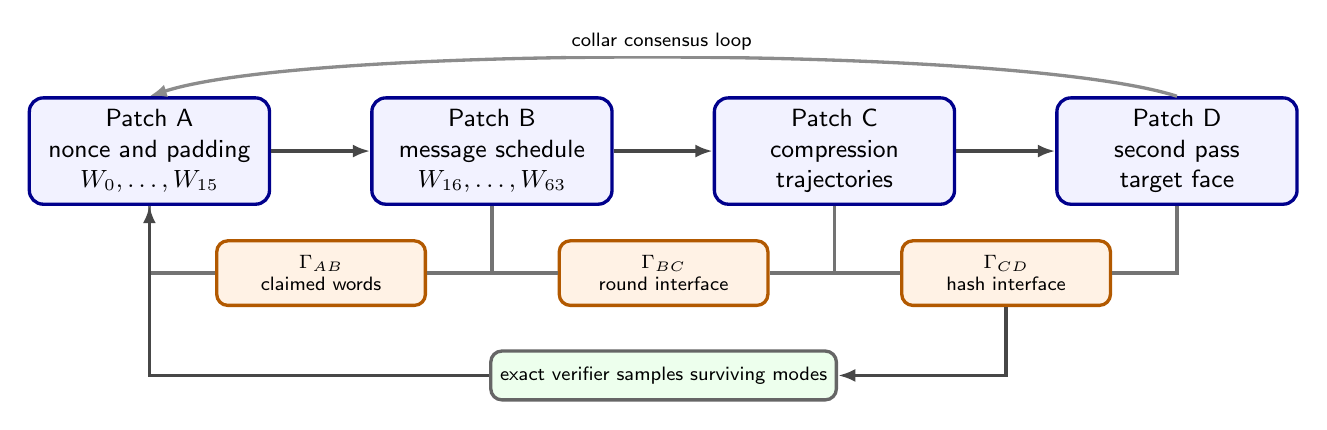
\begin{tikzpicture}[
  patch/.style={draw=blue!55!black, rounded corners=5pt, very thick,
    minimum width=3.05cm, minimum height=1.35cm, align=center,
    fill=blue!5, font=\sffamily\small},
  collar/.style={draw=orange!70!black, very thick, fill=orange!10,
    rounded corners=4pt, align=center, font=\sffamily\scriptsize,
    minimum width=2.65cm, minimum height=0.82cm},
  verifier/.style={draw=black!60, very thick, fill=green!7, rounded corners=4pt,
    align=center, font=\sffamily\scriptsize, minimum width=3.6cm,
    minimum height=0.62cm},
  flow/.style={-{Latex[length=2.2mm]}, very thick, draw=black!72},
  link/.style={very thick, draw=black!55}
]
\node[patch] (A) at (0,0) {Patch A\\nonce and padding\\\(W_0,\ldots,W_{15}\)};
\node[patch] (B) at (4.35,0) {Patch B\\message schedule\\\(W_{16},\ldots,W_{63}\)};
\node[patch] (C) at (8.70,0) {Patch C\\compression\\trajectories};
\node[patch] (D) at (13.05,0) {Patch D\\second pass\\target face};
\node[collar] (AB) at (2.18,-1.55) {\(\Gamma_{AB}\)\\claimed words};
\node[collar] (BC) at (6.53,-1.55) {\(\Gamma_{BC}\)\\round interface};
\node[collar] (CD) at (10.88,-1.55) {\(\Gamma_{CD}\)\\hash interface};
\node[verifier] (V) at (6.53,-2.85) {exact verifier samples surviving modes};

\draw[flow] (A.east) -- (B.west);
\draw[flow] (B.east) -- (C.west);
\draw[flow] (C.east) -- (D.west);

\draw[link] (A.south) |- (AB.west);
\draw[link] (B.south) |- (AB.east);
\draw[link] (B.south) |- (BC.west);
\draw[link] (C.south) |- (BC.east);
\draw[link] (C.south) |- (CD.west);
\draw[link] (D.south) |- (CD.east);

\draw[flow] (CD.south) |- (V.east);
\draw[flow] (V.west) -| (A.south);
\draw[flow, draw=black!45] (D.north) .. controls (11.0,1.35) and (2.0,1.35) ..
  node[above, font=\sffamily\scriptsize, fill=white, inner sep=2pt]{collar consensus loop} (A.north);
\end{tikzpicture}
}
\caption{The four-constraint-patch SHA-256d decomposition. Global satisfying assignments
are exactly local satisfying assignments that agree on all collars. OMEGA-I1
uses this graph as the scorebook and route program for a five-module physical
federation. The mathematical equivalence comes from the variable cover and
collar equalities.}
\label{fig:fourpatch}
\end{figure}

\begin{theorem}[Patch equalizer theorem]
\label{thm:equalizer}
Let
\[
\Sol_i=\{s_i\in\bits^{V_i}:E_i(s_i)=0\}
\]
be the local solution set of patch \(i\). Let \(\Sol_{\mathrm{collar}}\) be
the set of tuples
\[
(s_A,s_B,s_C,s_D)\in
\Sol_A\times\Sol_B\times\Sol_C\times\Sol_D
\]
whose restrictions agree on every collar:
\[
s_i|_{V_i\cap V_j}=s_j|_{V_i\cap V_j}.
\]
Then restriction gives a bijection between global zero-energy states of
\(E_A+E_B+E_C+E_D\) and \(\Sol_{\mathrm{collar}}\).
\end{theorem}

\begin{proof}
If \(s\) is a global zero-energy state, every nonnegative local energy is zero,
so \(s|_{V_i}\in\Sol_i\). Since all restrictions come from the same global
assignment, they agree on intersections. Thus \(s\) maps into
\(\Sol_{\mathrm{collar}}\).

Conversely, take a collar-consistent tuple
\((s_A,s_B,s_C,s_D)\). Collar consistency means that if a variable appears in
more than one patch, all patches assign it the same bit. Therefore the local
assignments glue to a unique global assignment \(s\in\bits^V\). Every local
energy is zero by \(s_i\in\Sol_i\), so \(E_A+E_B+E_C+E_D=0\). The two maps are
inverse by construction.
\end{proof}

This theorem is the formal content behind the phrase that bad candidates die at
collars. A collar mismatch certifies that a local assignment cannot glue to a
global satisfying assignment.

This is also why the OMEGA-I1 route can use different geometries without losing
the SHA proof. The physical chambers may have different bodies; they emit
decoded claims about the same variables and collars. If those decoded claims
agree and have zero local penalty, the equalizer theorem supplies the global SHA
witness. If they disagree, the disagreement is a syndrome for the next repair
pass.

\subsection{OMEGA-I1 physical deployment}

The optimized hardware target is OMEGA-I1: a five-module federation, not
a one-to-one four-chamber implementation of \(A,B,C,D\). The four-constraint-patch compiler
produces a scorebook, candidate grammar, collar residuals, and exact-verifier
interface. The OMEGA-I1 runtime executes that program on five host-routed
modules with the
same architecture used by the software reference and the contractor build package
described in this paper.
The public OMEGA educational guide gives a broader visual introduction to
chamber families, collars, and candidate-set narrowing \cite{OmegaEducationalGuide2026}.

\begin{center}
\begin{minipage}{\linewidth}
\centering
\small
\begin{tabular}{L{0.20\linewidth}L{0.20\linewidth}L{0.48\linewidth}}
\toprule
Compiler role & OMEGA-I1 module & SHA-256d purpose\\
\midrule
\(A/B\) source and early collars & \texttt{TOR-A} &
Nonce-stream recurrence, prefix-depth collars, and primary candidate-beam
generation.\\
\(A/B\) duplicate & \texttt{TOR-B} &
Independent duplicate of the recurrent stream for repeatability, ABBA, and
module-specific artifact rejection.\\
\(A/B/C\) search expansion & \texttt{TOR-C} &
Search-specialist torus for nonce-neighborhood expansion around near-prefix
or low-residual candidates.\\
\(C/D\) critic & \texttt{MIX-A} &
Asymmetric bit-slice critic for leading-zero windows, selected digest-byte
constraints, and mode-separation tests.\\
\(D\) verifier shadow & \texttt{ECH-A} &
Symmetric reference body for an independent SHA-prefix shadow before the final
host exact hash.\\
\bottomrule
\end{tabular}
\captionof{table}{OMEGA-I1 deployment of the four-constraint-patch SHA-256d compiler. The
physical architecture uses five 12-port modules because search, duplicate
repeatability, asymmetric criticism, and reference shadowing are different
hardware jobs.}
\label{tab:omega-i1-route}
\end{minipage}
\end{center}

The default optimized route is:
\[
\texttt{TOR-A/TOR-B}
\longrightarrow
\texttt{TOR-C}
\longrightarrow
\texttt{MIX-A}
\longrightarrow
\texttt{ECH-A}
\longrightarrow
\text{exact SHA-256d verifier}.
\]
All arrows in this route are host messages. OMEGA-I1 has no direct
module-to-module optical path, timing wire, or shared chamber power rail in the
contractor acceptance build. That constraint is useful: every boundary update is
recorded as a replayable scorebook transition with module IDs, firmware hashes,
coupling-matrix hashes, operator-probe hashes, input and output beam hashes, and
the host verifier receipt.

This five-module route is also the optimization surface. \texttt{TOR-A} and
\texttt{TOR-B} earn trust through statistical agreement. \texttt{TOR-C}
increases local candidate density around low-residual prefixes. \texttt{MIX-A}
rejects digest-window false positives under same-energy controls.
\texttt{ECH-A} preserves useful candidates under a different geometry before the
exact verifier spends hashes. A claimed lift that appears only after host
ranking, only in one torus duplicate, or only after exact-verifier selection is
outside the OMEGA-I1 hardware claim.

\subsection{How the federation searches many candidates in one settling event}

OMEGA-I1 uses a host-routed consensus search over optical candidate beams across
five chambers. A candidate beam is a recorded packet
\[
\mathcal B_t=\{(x,\rho,\phi,\sigma,\pi)\},
\]
where \(x\) is a candidate nonce or nonce-neighborhood descriptor, \(\rho\) is a
rank score, \(\phi\) is the decoded patch/collar residual, \(\sigma\) is the
module-local readout signature, and \(\pi\) is provenance: route ID, module ID,
drive program, decoder, firmware hash, and run time. The optical chamber is
responsible for changing the distribution of \(\mathcal B_t\). The host is
responsible for recording the transition and exact-checking any decoded nonce.

The phrase ``many candidates at the same time'' means that one drive/settle/read
cycle populates many optical paths, scattering histories, port-coupling modes,
and decoder branches before a digital verifier is called. The paper counts no
photon, analog microstate, or possible real-valued readout as a verified hash
unless the audited decoder emits a distinct verifier-ready candidate. The packet
size in the speedup formula, \(m_{\mathrm{pkt}}\), is the number of distinct
verifier-ready candidates emitted by the audited decoder after deduplication. A
larger effective mode envelope
\(N_{\mathrm{eff}}\) is useful only if it produces a larger audited
\(m_{\mathrm{pkt}}\), a larger verified bias \(\beta(k)\), or both.

Each stage has a different geometry because different failure modes need
different witnesses:

\begin{center}
\begin{minipage}{\linewidth}
\centering
\small
\setlength{\tabcolsep}{3pt}
\begin{tabular}{L{0.16\linewidth}L{0.22\linewidth}L{0.28\linewidth}L{0.24\linewidth}}
\toprule
Stage & Input & Physical job & Output message\\
\midrule
\texttt{TOR-A} &
Header or midstate scorebook, nonce grammar, collar weights &
Populate a recurrent nonce beam and expose prefix-depth collars &
Primary beam \(\mathcal B_A\), local residuals, port signature.\\
\texttt{TOR-B} &
Same scorebook under blinded labels or ABBA order &
Repeat the recurrent search in an independent duplicate torus &
Duplicate beam \(\mathcal B_B\), agreement and artifact checks.\\
\texttt{TOR-C} &
Consensus beam from \texttt{TOR-A/B} plus repair weights &
Expand neighborhoods around low-residual or near-prefix candidates &
Expanded beam \(\mathcal B_C\), repair deltas, new residuals.\\
\texttt{MIX-A} &
\(\mathcal B_C\), digest-window masks, selected bit-slice constraints &
Break degeneracies and reject false positives with asymmetric mixing &
Critic beam \(\mathcal B_M\), rejected modes, bit-slice residuals.\\
\texttt{ECH-A} &
\(\mathcal B_M\), target-face scorebook, reference geometry &
Shadow the survivors in a symmetric OPH reference body &
Reference beam \(\mathcal B_E\) for exact host SHA-256d.\\
\bottomrule
\end{tabular}
\captionof{table}{Executable OMEGA-I1 federation layout. Every arrow is a
host-recorded collar message instead of an unobserved optical link between
chambers.}
\label{tab:omega-i1-executable-route}
\end{minipage}
\end{center}

The host repair loop is explicit:

\begin{enumerate}
\item Compile the block template or midstate into a scorebook containing the
four-constraint-patch variables, collar masks, local penalties, route thresholds, and
decoder rules.
\item Drive \texttt{TOR-A} and \texttt{TOR-B} with matched or blinded scorebooks.
Decode \(\mathcal B_A\) and \(\mathcal B_B\). Keep only candidates or
neighborhoods whose collars agree above the duplicate-consensus threshold.
\item Treat duplicate disagreement as a syndrome. Increase weights on the failed
collars, lower trust in module-local artifacts, and rerun or route survivors to
\texttt{TOR-C}.
\item Let \texttt{TOR-C} perform search-neighborhood expansion around the
survivors. Accept the expansion only if the hard residual \(\Phi\) decreases or
if exact low-difficulty controls show a reproducible \(\beta(k)\) lift.
\item Route the expanded beam through \texttt{MIX-A}. The mixer may kill
candidates cheaply; inventing a hit is outside its role. Its output must improve
the exact-verifier hit rate at fixed pass rate under same-energy and
shuffled-label controls.
\item Route the critic survivors through \texttt{ECH-A}. The Echosahedron is the
reference shadow: a torus or mixer artifact tends to fail here. A candidate that
survives different geometry has a stronger consensus record.
\item Exact-check every serious decoded nonce with host SHA-256d. The exact
digest, leading-zero count, route transcript, and all control hashes go into the
run bundle.
\end{enumerate}

Consensus means intersection under repair. A candidate is better when
independent geometries keep sending compatible collar messages about it while
\(\Phi\) decreases. Repair means changing the next drive/scorebook from the
input syndrome. A good repair move can work without knowing the valid nonce in
advance; it only needs to make the next packet less inconsistent on the SHA-256d
collars and more enriched under the exact verifier.

\section{Observer-Screen Repair Dynamics}

OPH adds dynamics to the static equalizer. Patches carry private states,
collars expose shared observables, mismatch syndromes report disagreement, and
repair moves change local data to reduce the mismatch. The consensus paper
develops this as a finite repair system with a Lyapunov function
\cite{OPHConsensusCurrent}. For SHA-256d, use the following finite repair map.

Let \(G=(\{A,B,C,D\},E)\) be the patch graph and let
\[
\Phi(s_A,s_B,s_C,s_D)
=
\sum_{(i,j)\in E}
w_{ij}\,
d_{ij}\!\left(s_i|_{\Gamma_{ij}},s_j|_{\Gamma_{ij}}\right)
\;+\;
\sum_i \lambda_i E_i(s_i),
\]
where \(w_{ij},\lambda_i>0\) and \(d_{ij}\) is Hamming distance on the collar.
The first term punishes collar disagreement. The second term punishes local
gate violations.

In the OMEGA-I1 implementation, \(s_A,\ldots,s_D\) are not hidden claims about
the full analog state of a chamber. They are the hard-decoded route states
printed by the host after each module pass. The run bundle therefore contains
both layers: raw optical traces and the decoded \((s_A,s_B,s_C,s_D,\Phi)\)
record. The raw traces support operator-alignment and artifact audits. The
decoded record supports the SHA-256d equalizer and repair accounting.

\begin{proposition}[Finite repair termination]
\label{prop:repairtermination}
On a finite patch state space, any repair rule that commits only moves that
strictly decrease \(\Phi\) terminates after finitely many accepted moves.
\end{proposition}

\begin{proof}
The state space is finite and \(\Phi\) takes values in a finite subset of
\(\mathbb R_{\ge 0}\). A strictly decreasing sequence in a finite ordered set
must terminate.
\end{proof}

\begin{proposition}[Consensus equals solution under completeness]
\label{prop:repaircomplete}
Assume the repair rule is terminating, locally confluent, and complete in the
sense that every terminal state has \(\Phi=0\) whenever a zero-energy global
state exists in its connected repair component. Then every terminal state in
that component glues to a valid SHA-256d nonce, and the terminal normal form is
independent of repair order.
\end{proposition}

\begin{proof}
Termination and local confluence imply confluence by Newman's lemma. Hence each
state in the component has a unique normal form independent of repair order.
Completeness says the normal form has \(\Phi=0\). Thus all local energies vanish
and all collars agree. The Patch Equalizer Theorem then glues the local states
to a global zero-energy state of \(E_{\shaD,B,T}\). By
Theorem~\ref{thm:shaencoding}, the nonce coordinates are valid.
\end{proof}

The completeness assumption is the difficulty. Nonconvex constraint systems can
have traps. A successful physical solver either avoids those traps, escapes
them, or provides a measurable success probability large enough to beat
enumeration after exact verification.

\section{The Role of the OPH Pixel Constant \texorpdfstring{\(P\)}{P}}

The OPH papers use a dimensionless local pixel ratio
\[
P=\frac{a_{\mathrm{cell}}}{\ell_\star^2},
\]
where \(a_{\mathrm{cell}}\) is the microscopic screen-cell area and \(\ell_\star\)
is the OPH scale-readout length, displayed as the Planck length after the gravity row emits
\(G_{\mathrm{SI}}=c^3\ell_\star^2/\hbar\) \cite{OPHCompactCurrent,OPHScreenCurrent}. In the public OPH
release, \(P\) is selected by the fixed-point equation
\[
P=\varphi+\sqrt{\pi}\,\alpha_{\mathrm{em}}(0;P)
=\varphi+\frac{\sqrt{\pi}}{A_T(P)},
\qquad
\varphi=\frac{1+\sqrt5}{2},
\]
with reported solution
\[
P_\ast=1.630968209403959324879279847782648941\ldots.
\]

For the SHA-256d hardware instantiation, \(P\) is a dimensionless OPH design
target for geometry and coupling. It leaves the SHA-256 equations unchanged.
A \(P\)-calibrated
wave body is one whose normalized collar couplings, path-length ratios, and
extraction windows are tuned to the OPH fixed-point scale. In a toroidal or
microwave implementation, this means that the
dimensionless ratios
\[
\frac{R}{a},\qquad
\frac{a}{b},\qquad
\frac{L_j}{\lambda},\qquad
\frac{\kappa_{ij}}{\kappa_0}
\]
are selected from a small \(P_\ast\)-centered design family. In a photonic mesh,
it means that phase shifters, couplers, and nonlinear thresholds are tuned so
the realized coupling matrix \(\widehat K(P_\ast)\) approximates the intended
constraint matrix \(K_C\):
\[
\|\widehat K(P_\ast)-K_C\|\le \varepsilon_{\mathrm{geom}}.
\]

\begin{remark}[Geometry target]
All correctness theorems below depend on exact implementation of the
constraint Hamiltonian or exact return of a zero-energy state. The constant
\(P_\ast\) is part of the OPH interpretation and hardware calibration rule.
It fixes the geometry target. It is not, by itself, a mining receipt or an
operator-alignment proof. The proof comes from the implemented constraint
map, the measured operator bundle, and the exact verifier.
\end{remark}

\section{Wave and Hardware Encodings}

\subsection{Signed wave bits}

Use the signed encoding
\[
b\in\bits,\qquad \tilde b=(-1)^b\in\pmone.
\]
Then
\[
\widetilde{\neg b}=-\tilde b,\qquad
\widetilde{b\oplus c}=\tilde b\,\tilde c.
\]
The AND gate has signed output
\[
\widetilde{b\wedge c}
=\frac{1+\tilde b+\tilde c-\tilde b\tilde c}{2}.
\]
Equivalently, it is the threshold function
\[
\widetilde{b\wedge c}
=\sgn(\tilde b+\tilde c+1),
\]
with the convention \(\sgn(u)=+1\) for \(u>0\) and \(-1\) for \(u<0\). The carry
bit of a full adder is a majority gate, also a threshold:
\[
\widetilde{\operatorname{carry}(b,c,d)}
=\sgn(\tilde b+\tilde c+\tilde d).
\]
Thus rotations and permutations are geometry, XOR is phase-sensitive mixing,
and carries require a nonlinear threshold or an equivalent measurement-feedback
resource.

\begin{lemma}[Passive linear optics no-go for exact SHA-256 logic]
\label{lem:linearno}
A purely passive linear wave network with linear readout cannot exactly
implement a universal SHA-256 gate layer on signed bits. In particular, it
cannot exactly implement AND or full-adder carry for all inputs.
\end{lemma}

\begin{proof}
A passive linear network maps input amplitudes \(u\) to \(Lu\) for a linear
operator \(L\). Any single output amplitude is an affine-linear function of the
input amplitudes after adding a constant bias mode. On signed inputs
\((a,b)\in\pmone^2\), AND in signed form is
\[
f(a,b)=\frac{1+a+b-ab}{2}.
\]
The term \(-ab/2\) is not affine-linear. More directly, if
\(f(a,b)=c_0+c_1a+c_2b\), the four truth-table equations give
\[
\begin{aligned}
c_0+c_1+c_2&=1,\\
c_0+c_1-c_2&=1,\\
c_0-c_1+c_2&=1,\\
c_0-c_1-c_2&=-1,
\end{aligned}
\]
whose first three equations imply \(c_0=1,c_1=c_2=0\), contradicting the fourth.
Full-adder carry contains the same threshold nonlinearity. SHA-256 uses modular
addition, hence carry. Therefore passive linear optics alone is insufficient.
\end{proof}

KLM-style linear optical quantum computation uses single photons, detection,
ancillas, feedback, and effective measurement-induced nonlinearity
\cite{KLM2001}. Classical optical Ising machines use nonlinear oscillators or
measurement feedback for the same reason \cite{Yamamoto2017,CIM100k2021}.

\subsection{Classical OMEGA-I1 wave variant}

The OMEGA-I1 classical variant is LED-first and contractor-buildable. Each
module is an enclosed 12-port optical body with co-located red LED source and
BPW34-class detector channels, an RP2350-class USB controller, bounded LED
current, and exact host-side records. Laser, OPO, strict same-electrode
transmit/receive, and HAPTIC-style upgrades are separate hardware targets. They
are outside the baseline used for the SHA-256d architecture in this paper
and outside the OMEGA-I1 acceptance build.

The physical computation is therefore a host-routed candidate-enrichment loop.
The chamber modules expose coupling maps, edge responses, settle traces,
operator probes, and candidate beams. The host applies the four-constraint-patch scorebook,
routes beams between modules, and exact-checks serious candidates.

\subsection{The solver contract for fixed OMEGA shapes}

A solver in this paper is a physical sampler with a strict contract. The input is
a scorebook: variables, local penalties, collar masks, drive weights, decoder
rules, repair thresholds, and an exact verifier. The output is a candidate beam:
decoded nonce assignments or nonce-neighborhood assignments with residuals,
provenance, and control receipts. The chamber earns the word solver only when
the decoded beam is enriched under the exact verifier at fixed controls.
There is no infinite-improbability drive hidden in the word solver: lift means
verifier-visible enrichment under audited controls.

This is how OMEGA-I1 can be general compute despite fixed chamber shapes. The
printed body supplies a reusable coupling basis. The program is the port drive,
label map, scorebook, decoder, route order, feedback rule, and host-side repair
logic. A torus chamber can therefore run a SHA-256d scorebook, a kHeavyHash
scorebook, or a small SAT scorebook by changing the imposed variables and collar
tests while keeping the same measured port body. The body is the analog
substrate; the scorebook is the program.

For SHA-256d, the LED OMEGA-I1 build is a photonic constraint solver. Light
transport explores many coupled path modes in one settle/read event, nonlinear
ports and feedback supply the carry and target commitments, and the host keeps
only decoded candidates whose collars and exact hashes improve the audited
distribution. In a single-photon Omega version, the same scorebook becomes a
quantum solver: occupation states encode candidate assignments, interferometric
paths carry amplitude and phase, and detection plus feed-forward supplies the
nonlinear commitments. The quantum claim comes from coherent occupation-state
dynamics and coherence receipts; Grover-style claims require a separate
reversible-oracle and diffusion audit.

\begin{figure}[t]
\centering
\resizebox{0.98\linewidth}{!}{%
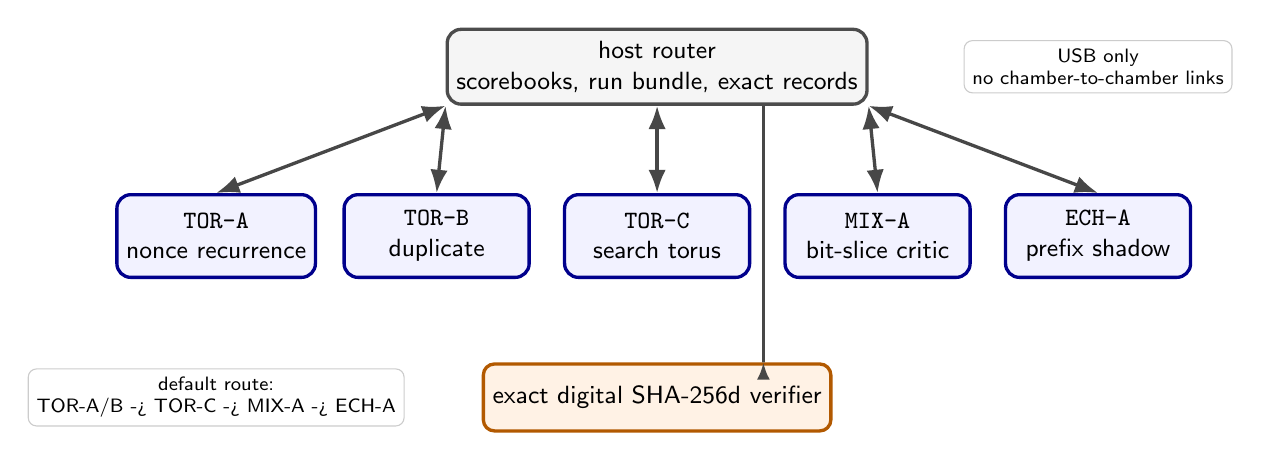
\begin{tikzpicture}[
  module/.style={draw=blue!55!black, rounded corners=5pt, very thick,
    align=center, fill=blue!5, minimum width=2.35cm, minimum height=1.05cm,
    font=\sffamily\small},
  host/.style={draw=black!70, rounded corners=5pt, very thick,
    align=center, fill=gray!8, minimum width=4.4cm, minimum height=0.95cm,
    font=\sffamily\small},
  verifier/.style={draw=orange!70!black, very thick, align=center,
    fill=orange!10, rounded corners=4pt, minimum width=3.7cm, minimum height=0.85cm,
    font=\sffamily\small},
  labelbox/.style={draw=black!20, rounded corners=3pt, fill=white,
    inner sep=3pt, align=center, font=\sffamily\scriptsize},
  usb/.style={<->, >=Latex, very thick, draw=black!72},
  flow/.style={-{Latex[length=2.2mm]}, very thick, draw=black!72}
]
\node[host] (host) at (5.6,2.15) {host router\\scorebooks, run bundle, exact records};
\node[module] (tora) at (0,0) {\texttt{TOR-A}\\nonce recurrence};
\node[module] (torb) at (2.8,0) {\texttt{TOR-B}\\duplicate};
\node[module] (torc) at (5.6,0) {\texttt{TOR-C}\\search torus};
\node[module] (mixa) at (8.4,0) {\texttt{MIX-A}\\bit-slice critic};
\node[module] (echa) at (11.2,0) {\texttt{ECH-A}\\prefix shadow};
\node[verifier] (verifier) at (5.6,-2.05) {exact digital SHA-256d verifier};
\node[labelbox] (usbnote) at (11.2,2.15) {USB only\\no chamber-to-chamber links};
\node[labelbox] (route) at (0,-2.05) {default route:\\TOR-A/B -> TOR-C -> MIX-A -> ECH-A};

\draw[usb] (host.south west) -- (tora.north);
\draw[usb] (host.south west) -- (torb.north);
\draw[usb] (host.south) -- (torc.north);
\draw[usb] (host.south east) -- (mixa.north);
\draw[usb] (host.south east) -- (echa.north);
\coordinate (hostverify) at ($(host.south)+(1.35,0)$);
\coordinate (verifytap) at ($(verifier.north)+(1.35,0)$);
\draw[flow] (hostverify) -- ++(0,-0.8) |- (verifytap);
\end{tikzpicture}
}
\caption{OMEGA-I1 SHA-256d architecture. The five optical modules are separate
USB nodes. The host owns the route, run bundle, scorebooks, and exact
SHA-256d verifier. The physical modules enrich and filter candidate beams; the
host records every boundary transition and performs final verification.}
\label{fig:hardware}
\end{figure}

An idealized diode-threshold model is:
\[
u_{\mathrm{out}}=\sgn\!\left(\sum_j \eta_j u_j-\theta\right),
\]
where the sign is physically approximated by a biased nonlinear I-V curve or a
lasing threshold. A real device has finite slope, jitter, shot noise, thermal
noise, and drift. Let the implemented threshold be \(D_{\theta,\delta}\), where
\(\delta\) bounds the uncertain switching band. Exact Boolean operation is
certified only when every legal input has margin \(>\delta\).

\begin{proposition}[Noise-margin condition]
If every nonlinear gate in a physical SHA-256d solver has input margin at least
\(\gamma>0\), implementation error at most \(\varepsilon<\gamma\), and feedback
keeps perturbations below \(\gamma-\varepsilon\) before the subsequent
thresholding event, then the physical gate layer has the same Boolean truth
table as the ideal gate layer.
\end{proposition}

\begin{proof}
For each threshold gate, legal inputs lie at distance at least \(\gamma\) from
the switching surface. Perturbing the threshold argument by at most
\(\varepsilon<\gamma\) cannot cross the switching surface, so the sign is
unchanged. The feedback condition preserves the same margin for the following layer.
Induction over the gate layers gives equality of the physical and ideal truth
tables.
\end{proof}

\subsection{OMEGA-I1 boundary and operator alignment}

The Omega hardware program requires more evidence than a verified hash for the
physical claim. An exact verifier proves that a candidate nonce works. Chamber
alignment with the SHA-256d operator requires separate controls against parser
bias, host loops, and accidental transport channels.

Let \(L_T\) be the finite task operator for the target predicate, let
\(K_{\mathrm{model}}\) be the modeled chamber operator in a declared basis, and
let \(K_{\mathrm{phys}}\) be the measured physical port operator in the same
normalization. The Omega commutator gate asks whether the chamber approximately
preserves the task structure:
\[
\lVert [K_{\mathrm{model}},L_T]\rVert\le \epsilon .
\]
Physical realization then has its own error budget.

\begin{proposition}[Bounded-commutator transfer]
\label{prop:commutatortransfer}
If
\[
\lVert [K_{\mathrm{model}},L_T]\rVert\le \epsilon,\qquad
\lVert K_{\mathrm{phys}}-K_{\mathrm{model}}\rVert\le \delta,
\]
in a common operator norm, then
\[
\lVert [K_{\mathrm{phys}},L_T]\rVert
\le
\epsilon+2\delta\lVert L_T\rVert .
\]
\end{proposition}

\begin{proof}
Write \(K_{\mathrm{phys}}=K_{\mathrm{model}}+\Delta\). Then
\[
[K_{\mathrm{phys}},L_T]=[K_{\mathrm{model}},L_T]+[\Delta,L_T].
\]
The triangle inequality gives the first term as \(\epsilon\), and
\(\lVert[\Delta,L_T]\rVert\le
\lVert\Delta L_T\rVert+\lVert L_T\Delta\rVert
\le 2\delta\lVert L_T\rVert\).
\end{proof}

This proposition is a design gate. A solved-SHA claim requires the following
printed evidence: the
basis, normalization, task operator, modeled operator, measured port operator,
operator-probe data, settle traces, edge responses, and exact-verifier
receipts for the same run bundle.

\subsection{Sampler-class SHA-256d operating program}

The SHA-256d hardware plan is sampler-class. It aims to enrich the candidate
stream before exact verification. Grover-class quadratic amplification and
universal-NP oracle claims require separate evidence. The operating program has
four roles:

\begin{enumerate}
\item broad mode population, so the body explores many nonce-conditioned modes;
\item in-substrate mode-leak selection, where threshold and hysteresis supply
the load-bearing nonlinear commitment for AND, \(\Maj\), carry, and target
faces;
\item closed-loop transmit/receive feedback, where collar syndromes change the
next physical drive instead of merely logging telemetry;
\item MCU warm-loop transport, which raises packet rate and lowers USB or host
latency without taking over the search.
\end{enumerate}

The distinction matters. Firmware transport may increase \(m_{\mathrm{pkt}}\) by
moving candidates faster. Physical bias \(\beta\) rises only when the chamber
changes the distribution of exact-verifier outcomes. If the MCU
performs the search that the chamber was supposed to perform, the optical claim
has evaporated. The finite gate stack is therefore
\[
\begin{aligned}
&\texttt{EDGE\_BRACKETED}\to
\texttt{EDGE\_POLARITY\_LOCKED}\\
&\to \texttt{NONLINEAR\_COMMITMENT\_ALIVE}\to
\texttt{TRUTH\_LIFT}\\
&\to \texttt{POOL\_SHARE\_LIFT}\to \texttt{BLOCK}.
\end{aligned}
\]
OMEGA-I1 assigns \texttt{TOR-A} and \texttt{TOR-B} to duplicate recurrent
streams, \texttt{TOR-C} to search-specialist expansion, \texttt{MIX-A} to
bit-slice criticism, and \texttt{ECH-A} to reference shadowing. The digital
reference model uses the same full-five route and its single, pair, subset, and
shuffled controls as a guardrail before hardware escalation.

\subsection{Single-photon quantum variant}

The quantum build uses single-photon occupation states in a linear-optical
processor. A logical bit can be encoded in dual rail, time bins, or paths:
\[
|0_L\rangle=|1\rangle_0|0\rangle_1,\qquad
|1_L\rangle=|0\rangle_0|1\rangle_1.
\]
Beam splitters, phase shifters, delay lines, switches, detectors, ancilla
photons, and feed-forward implement the gate set. KLM shows that this resource
set can be universal for quantum computation in principle \cite{KLM2001}. In
the OPH reading, the same chamber geometry carries the mode graph, while the
single-photon occupation basis supplies quantum amplitude, phase, and
measurement.

The candidate register is prepared as
\[
|s\rangle=\frac{1}{\sqrt N}\sum_{x\in\bits^n}|x\rangle.
\]
The reversible SHA-256d oracle computes the mining predicate into a work qubit
and then uncomputes its scratch space:
\[
U_V|x\rangle|q\rangle|0^r\rangle
=|x\rangle|q\oplus V(x)\rangle|0^r\rangle.
\]
With a phase kickback qubit, this becomes the phase oracle
\[
O_V|x\rangle=(-1)^{V(x)}|x\rangle.
\]
One Grover step is
\[
G=(2|s\rangle\langle s|-I)\,O_V.
\]
The photonic device must implement:

\begin{itemize}
\item heralded single-photon state preparation for the candidate, ancilla, and
phase-kickback registers;
\item a reversible SHA-256d circuit compiled into interferometers, switches,
measurement-induced nonlinear gates, and feed-forward;
\item a diffusion/reflection network implementing \(2|s\rangle\langle s|-I\);
\item coherent repetition of the oracle and diffusion layers for
\(\Theta(\sqrt{N/M})\) Grover steps;
\item final number-resolving or threshold detection followed by exact classical
verification of the measured candidate.
\end{itemize}

For a leading-zero target with success probability \(p=2^{-k}\), the ideal
Grover iteration count is
\[
Q_{\mathrm{G}}(k)\approx \frac{\pi}{4}2^{k/2},
\]
with query speedup
\[
S_{\mathrm{G}}(k)\approx \frac{2^k}{Q_{\mathrm{G}}(k)}
=\frac{4}{\pi}2^{k/2}.
\]
The gain is quadratic in query count. The wave-overlap zero-energy endpoint has
a different scaling: a physical fixed point can represent a valid nonce in one
settling event. Resource estimates for generic SHA-256
preimage search remain enormous. Amy et al. estimate a SHA-256 preimage attack
requiring approximately \(2^{153.8}\) surface-code cycles and \(2^{12.6}\)
logical qubits, or \(2^{166.4}\) logical-qubit-cycles \cite{AmyEtAl2016}.
The Omega/Karma hardware described here sits outside this Grover resource set.
The Grover rows in this paper are comparison baselines unless a separate audit
prints a reversible oracle, diffusion operator, maintained coherence, and
quadratic scaling receipts.

\FloatBarrier
\section{Keccak and SHA-3 Variant}

SHA-256 and Keccak/SHA-3 are different hash families. SHA-3 is standardized in
FIPS 202 and is based on the Keccak permutation \cite{NISTFIPS202}. The same
physical design vocabulary can describe Keccak. The gate map differs.

\begin{center}
\begin{minipage}{\linewidth}
\centering
\begin{tabular}{lll}
\toprule
Keccak step & Logical operation & Geometric or physical encoding\\
\midrule
\(\theta\) & column parity XOR & phase-sensitive mixing / multiplier nodes\\
\(\rho\) & bit rotation & calibrated delay lines\\
\(\pi\) & lane permutation & routing and crossovers\\
\(\chi\) & nonlinear row update & threshold, diode, Kerr, or measurement feedback\\
\(\iota\) & round-constant XOR & fixed phase mask or sign flip\\
\bottomrule
\end{tabular}
\captionof{table}{Keccak/SHA-3 physical encoding dictionary. The nonlinear \(\chi\) step
has the same resource-accounting burden as modular carries in SHA-256.}
\label{tab:keccak}
\end{minipage}
\end{center}

Routing, rotations, and XOR-like phase relations are natural for waves.
Nonlinear Boolean steps require a nonlinear physical process or measurement
feedback. A Keccak implementation has to specify the \(\chi\) layer
with the same care that a SHA-256 implementation specifies carries.

Kaspa is useful here for a mechanical reason: its proof-of-work kernel is close
to the physics. kHeavyHash has the form
\[
\operatorname{kHH}
=
\operatorname{SHA3}(\mathrm{prepow},t,n)
\longrightarrow
M_{64\times64}\text{ nibble multiply}
\longrightarrow
\operatorname{SHA3}(\cdot),
\]
Its most chamber-friendly portion is a matrix operator bracketed by Keccak
permutations. Linear mixing, routing, and phase transport map naturally to a
wave body, while the \(\chi\) layer localizes the nonlinear part that the
ports must supply. The 2026-05-05 firmware handoff records a bit-exact
chamber-plus-MCU decomposition: full kHeavyHash matched the digital reference
on \(30/30\) tests, the SHA3 chamber-plus-MCU path matched Python hashlib, and
the local-quadratic \(\chi\) form matched textbook \(\chi\). SHA-256d has a different nonlinear core:
word additions, carries, \(\Ch\), and \(\Maj\). The four-constraint-patch map above is the
corresponding SHA-256d compiler target.

\FloatBarrier
\section{Optical Proof-of-Work Prototype}

The OPH/Karma optical proof-of-work prototype uses the same low-cost
optical-supercomputer surface as the OMEGA-I1 line: a clear wave body, RP2350 or
RP2040 control, reversible optical ports, firmware bring-up, and verification
steps \cite{OmegaOpticalSupercomputer2026}. It was not an OMEGA-I1 run. It is
used here as precursor evidence for optical candidate enrichment, not as a
measurement of the five-chamber SHA-256d route.

The OPH/Karma prototype has mined Kaspa kHeavyHash pool shares on the optical
candidate path. The optical chamber proposes candidates; host-side kHeavyHash
verification checks them before pool submission. An internal mining receipt log
records a Cedric Kaspa pool run in which optical candidates received pool
acknowledgements. The run log records:

\begin{itemize}
\item \(1649\) submitted optical candidates;
\item \(8\) accepted optical share responses;
\item \(99\) submitted optical candidates without a returned pool response;
\item best host-recomputed leading-zero quality near \(21\);
\item best reported share difficulty near \(2.93\times 10^6\).
\end{itemize}

Separately, a May 6, 2026 shuffle-replay audit of the CASCADE/chord-promote
output recorded
\[
\widehat\beta(k)=
\{14.75\text{ at }k=4,\;229\text{ at }k=8,\;886\text{ at }k=10,\;
2{,}434\text{ at }k=12\},
\]
with mean leading-zero count \(11.83\) for the chamber-selected stream versus
\(0.92\) for random replay. In this notation, \(\widehat\beta(k)\) is the
observed exact-verifier success rate for the event \(\mathrm{lz}\ge k\), divided
by the uniform-random rate \(2^{-k}\). The exact headline number used in this
comparison lane is therefore \(\widehat\beta(12)=2{,}434\), meaning that
\(\mathrm{lz}\ge12\) candidates appeared \(2{,}434\) times the uniform-random
baseline in that selected stream. The boundary is important:
this is a controlled candidate-enrichment result on the chord-promote output,
not a final pool-rate or block-win result, and not evidence that the same slope
continues to network difficulty.

The same log also records the boundary conditions. A CPU pool baseline
established the pool contract. During the optical acceptance run, CPU workers
also contributed to wallet-level flow. A solo audit on May 2, 2026 recorded stable
operation, host verification, and share logging. It also recorded
host-verified leading-zero counts near random expectation and weak correlation
between board-local leading-zero reports and host recomputation.

The prototype closes a proof-of-work loop: optical candidate generation, exact
hash verification, and pool submission. Its boundary conditions are part of the
claim. The accepted-share log supports a real external-verifier path for
kHeavyHash/Kaspa, while the solo audit keeps the stronger enrichment claim open.
The SHA-256d construction sets the Bitcoin operator map for the same physical
search cascade. SHA-256d claims pass only through the operator-alignment and
per-distinct-enrichment gates above.

\section{Speedup Accounting}

\begin{theorem}[Candidate-enrichment work reduction]\label{thm:candidate-enrichment}
Let \(V(x)\in\{0,1\}\) be an exact verifier. Let \(U\) be the baseline candidate distribution and
\(Q\) the chamber-conditioned candidate distribution. Define
\[
p_U=\Pr_{x\sim U}[V(x)=1],
\qquad
p_Q=\Pr_{x\sim Q}[V(x)=1],
\qquad
B=\frac{p_Q}{p_U}.
\]
If \(B>1\), the expected number of exact verifier calls to find a valid candidate drops from
\[
\mathbb E_U[N]=\frac{1}{p_U}
\]
to
\[
\mathbb E_Q[N]=\frac{1}{p_Q}=\frac{1}{B p_U}.
\]
Thus the verifier-work reduction factor is exactly the measured enrichment \(B\). This theorem is
a distributional lift statement under an exact verifier, not a complexity-class theorem and not a
claim that arbitrary hard problems become easy.
\end{theorem}

\begin{proof}
Verifier calls are Bernoulli trials with success probabilities \(p_U\) and \(p_Q\). The waiting
time to the first success is geometric with expectation \(1/p\). Substituting
\(p_Q=Bp_U\) gives the result.
\end{proof}

Let \(R_{\mathrm{hash}}\) be a classical exact-verifier rate in hashes per
second, \(p=|T|/2^{256}\) the target fraction, and \(q\) the probability that a
physical candidate is valid after exact verification. An unbiased random
candidate stream has \(q=p\). A physical sampler has bias factor
\[
\beta=\frac{q}{p}.
\]
If each physical settling event costs time \(T_{\mathrm{settle}}\) and produces
\(m_{\mathrm{pkt}}\) independently verified candidates, the expected physical
time per valid nonce is
\[
\mathbb E[T_{\mathrm{phys}}]
=\frac{T_{\mathrm{settle}}}{1-(1-q)^{m_{\mathrm{pkt}}}}
\approx\frac{T_{\mathrm{settle}}}{m_{\mathrm{pkt}}\beta p}.
\]
The approximation is the cryptographic-target regime \(q\ll1\).
A classical miner using exact hashes has
\[
\mathbb E[T_{\mathrm{class}}]=\frac{1}{R_{\mathrm{hash}}p}.
\]
Thus the operational speedup is
\[
S=\frac{\mathbb E[T_{\mathrm{class}}]}{\mathbb E[T_{\mathrm{phys}}]}
\approx\frac{m_{\mathrm{pkt}}\beta}{R_{\mathrm{hash}}T_{\mathrm{settle}}}.
\]
The speedup has four measurable inputs: verifier rate, physical settling time,
packet size, and candidate bias. For OMEGA-I1, \(m_{\mathrm{pkt}}\) counts
distinct candidates that exit the full selected route. Raw LED emission counts
from a single module are excluded. A high bias loses value if settling is slow.
The Kaspa comparison lane supplies one historical candidate-bias datum,
\(\widehat\beta(12)=2{,}434\), measured on chord-promote output after
shuffle-replay. Equivalently, for the \(k=12\) exact-verifier predicate,
the selected stream's estimated success probability was \(2{,}434\times2^{-12}\)
instead of \(2^{-12}\). It does not by itself determine SHA-256d speedup,
because the operator, route, packet size, settle time, and high-\(k\) scaling
must be remeasured under the SHA-256d scorebook.
Against a classical verifier running at \(R_{\mathrm{hash}}\), the sampler wins
only when
\[
m_{\mathrm{pkt}}\beta>R_{\mathrm{hash}}T_{\mathrm{settle}}.
\]
At \(R_{\mathrm{hash}}=4.73\times10^{14}\,\mathrm{H/s}\) and
\(T_{\mathrm{settle}}=100\,\mathrm{ns}\), that threshold is
\(4.73\times10^7\). This is the practical optimization target: increase packet
size, increase verified bias, or reduce settle time. In OMEGA-I1, this product
must be measured at the full route output, not inferred from a single chamber's
raw optical mode count. The exact verifier stays in the loop.

\begin{center}
\begin{minipage}{\linewidth}
\centering
\begin{tabular}{L{0.24\linewidth}L{0.26\linewidth}L{0.38\linewidth}}
\toprule
Regime & Formal speedup & Required claim\\
\midrule
Classical ASIC enumeration & baseline \(1\) & exact SHA-256d per candidate\\
Single-photon Grover search & \(\frac{4}{\pi}\sqrt{N/M}\) query speedup &
reversible oracle, diffusion, coherence, fault tolerance\\
Wave-overlap sampler & \(m_{\mathrm{pkt}}\beta/(R_{\mathrm{hash}}T_{\mathrm{settle}})\) &
measured packet size and candidate bias after exact verification\\
Exact wave-overlap oracle & \(1/(R_{\mathrm{hash}}pT_{\mathrm{settle}})\) &
proof or measurement that terminal states are zero-energy solutions\\
\bottomrule
\end{tabular}
\captionof{table}{Speedup accounting. The wave-overlap sampler row uses measured packet
size and candidate bias after exact verification. The exact wave-overlap row is
the conditional endpoint of the physical construction, separate from measured
bench performance.}
\label{tab:speedups}
\end{minipage}
\end{center}

For a leading-zero target \(p=2^{-k}\), the exact wave-overlap endpoint has
\[
T_{\mathrm{zero}}(k)\approx T_{\mathrm{settle}},\qquad
S_{\mathrm{zero}}(k;R_{\mathrm{hash}},T_{\mathrm{settle}})
=\frac{2^k}{R_{\mathrm{hash}}T_{\mathrm{settle}}}.
\]
The single-photon Grover variant has
\[
Q_{\mathrm{G}}(k)\approx\frac{\pi}{4}2^{k/2},\qquad
S_{\mathrm{G}}(k)\approx\frac{4}{\pi}2^{k/2}.
\]
The wave-overlap sampler sits between these two limits. Its measured speed is
set by \(m_{\mathrm{pkt}}\beta\), the number of independently checked candidates per
settling event times the verified enrichment over random search. Firmware that
only improves transport raises \(m_{\mathrm{pkt}}\); only a changed
exact-verifier distribution raises \(\beta\).

For a concrete wall-clock baseline, take Bitmain's ANTMINER S21 XP Hyd
specification: SHA-256 mining at \(473\,\mathrm{TH/s}\), \(5676\,\mathrm{W}\),
and \(12.0\,\mathrm{J/TH}\) \cite{BitmainS21XPHyd2024}. Thus
\[
R_{\mathrm{ASIC}}=4.73\times10^{14}\ \mathrm{H/s}.
\]
An aggressive hydro reference is Auradine's AH3880 at up to
\(600\,\mathrm{TH/s}\) \cite{AuradineAH38802025}. Using \(600\,\mathrm{TH/s}\)
instead of \(473\,\mathrm{TH/s}\) multiplies the S21-based wall-clock
multipliers below by \(473/600\simeq0.79\). For a \(k\)-bit leading-zero target,
\[
T_{\mathrm{ASIC}}(k)=\frac{2^k}{R_{\mathrm{ASIC}}}.
\]
For a physical method with time \(T_{\mathrm{phys}}\), the ASIC-relative
multiplier is \(T_{\mathrm{ASIC}}(k)/T_{\mathrm{phys}}\). The following table is
a sensitivity calculation for proposed regimes, with no SHA-256d bench
measurement attached.

\begin{center}
\begin{minipage}{\linewidth}
\centering
\scriptsize
\setlength{\tabcolsep}{3pt}
\begin{tabular}{@{}L{0.18\linewidth}L{0.27\linewidth}L{0.22\linewidth}L{0.20\linewidth}@{}}
\toprule
Variant & Estimate inputs & Internal reduction & Wall-clock multiplier versus S21 XP Hyd\\
\midrule
High-end ASIC baseline & Bitmain S21 XP Hyd:
\(R_{\mathrm{ASIC}}=4.73\times10^{14}\,\mathrm{H/s}\) &
ordinary enumeration & \(1\times\)\\
Hypothetical wave-overlap sampler & \(m_{\mathrm{pkt}}\beta=10^9\),
\(T_{\mathrm{settle}}=100\,\mathrm{ns}\) &
candidate-value multiplier \(10^9\) per settling event &
\(2.1\times10^1\times\)\\
Exact wave-overlap endpoint & \(k=32\),
\(T_{\mathrm{settle}}=100\,\mathrm{ns}\) &
\(2^{32}\) trials to one settling event &
\(9.1\times10^1\times\)\\
Exact wave-overlap endpoint & \(k=64\),
\(T_{\mathrm{settle}}=100\,\mathrm{ns}\) &
\(2^{64}\) trials to one settling event &
\(3.9\times10^{11}\times\)\\
Exact wave-overlap endpoint & \(k=80\),
\(T_{\mathrm{settle}}=100\,\mathrm{ns}\) &
\(2^{80}\) trials to one settling event &
\(2.6\times10^{16}\times\)\\
Single-photon Grover & 32-bit nonce,
\(Q_G\approx(\pi/4)2^{16}\), \(T_G=1\,\mathrm{ns}\) &
coarse \(2^{16}=65{,}536\times\);
exact \(8.3\times10^4\times\) query reduction &
\(1.8\times10^{-1}\times\)\\
Single-photon Grover & \(k=64\),
\(Q_G\approx(\pi/4)2^{32}\), \(T_G=1\,\mathrm{ns}\) &
\(5.5\times10^9\times\) query reduction &
\(1.2\times10^4\times\)\\
\bottomrule
\end{tabular}
\captionof{table}{Numerical speedup estimates against a concrete high-end ASIC.
The ASIC baseline is Bitmain's \(473\,\mathrm{TH/s}\) S21 XP Hyd. Wave rows use
\(S=m_{\mathrm{pkt}}\beta/(R_{\mathrm{ASIC}}T_{\mathrm{settle}})\) for samplers and
\(S=2^k/(R_{\mathrm{ASIC}}T_{\mathrm{settle}})\) for the conditional exact
endpoint.
Single-photon rows use \(T_{\mathrm{phys}}=Q_G T_G\) with a \(1\,\mathrm{ns}\)
oracle-cycle estimate; these rows scale inversely with \(T_G\) and omit
fault-tolerance overhead.}
\label{tab:numericalspeedups}
\end{minipage}
\end{center}

Query reduction and wall-clock multiplier are separated because the ASIC
baseline evaluates \(4.73\times10^5\) hashes during a \(1\,\mathrm{ns}\) optical
cycle. The familiar \(65{,}536\times\) Grover number is the square-root
reduction for a 32-bit nonce space. At \(k=64\), the same \(1\,\mathrm{ns}\)
single-photon cycle gives a \(1.2\times10^4\times\) wall-clock multiplier
against the S21 XP Hyd baseline. In the exact wave-overlap endpoint, one
settling event supplies the candidate that ordinary enumeration would expect
after \(2^k\) trials.

\begin{theorem}[Physical-oracle consequence]
\label{thm:oracle}
Assume a uniform family of physical devices \(D_C\) can be constructed from any
Boolean circuit \(C\) in polynomial design time and polynomial physical
resources, and that \(D_C\) returns a satisfying assignment whenever one exists,
with bounded error, in polynomial physical time. Then NP search problems are
polynomial-time solvable in that physical model.
\end{theorem}

\begin{proof}
By Cook-Levin and the standard reduction picture, any NP witness-checking
problem has a polynomial-size Boolean circuit \(C_x(w)\) whose satisfying
assignments are witnesses \cite{Cook1971,Karp1972}.
Construct \(D_{C_x}\) and run it. By assumption, it returns a satisfying
witness in polynomial physical time when one exists, with bounded error.
\end{proof}

\begin{corollary}[Relation to classical complexity]
Theorem~\ref{thm:oracle} is a statement about the physical model. A classical
Turing-machine collapse follows if the device family admits polynomial-time
Turing simulation with the same bounded error.
\end{corollary}

The OPH blog essay uses the observer-screen slogan for this statement
\cite{OPHBlogPNP}.

The OMEGA-I1 claim boundary in this paper deliberately stops short of this
theorem's premise.
OMEGA-I1 can support sampler-class candidate enrichment, operator-probe
evidence, and exact-verifier receipts. By itself, OMEGA-I1 leaves the uniform
polynomial-time solver premise for arbitrary NP circuits unestablished.

Physical complexity questions of this kind have a classical literature in
analog computation and physical NP-complete proposals
\cite{VergisSteiglitzDickinson1986,Aaronson2005}.

\section{Public Evidence Protocol}

The Kaspa evidence records the physical path at accepted-share level. A public
SHA-256d cryptography submission needs the same class of evidence in a form
external readers can replay. The minimum protocol is:

\begin{enumerate}
\item Pre-register the block-header templates, target strengths \(k\), run
durations, stopping rules, and acceptance predicates.
\item Print the run tuple: route ID, ordered stage modules, board identifiers,
chamber identifiers, firmware hashes, compiler hash, scorebook hashes, wire
format, drive regime, receive regime, scorer, verifier, and duration.
\item Store raw timing traces, raw port readings, raw candidate nonces, and the
hard-decoded patch/collar residual \(\Phi\) before exact verification.
\item Verify every distinct candidate with an independent SHA-256d
implementation for the Bitcoin target, or with independent kHeavyHash for the
Kaspa comparison lane. Report the exact digest and leading-zero count for every
hit.
\item Report the number of distinct candidates \(N_{\mathrm{dist}}\), duplicate
rate, number of successes \(S\), expected random baseline
\(N_{\mathrm{dist}}p\), and the bias estimator
\[
\widehat\beta(k)=\frac{S}{N_{\mathrm{dist}}p}.
\]
\item Compute a binomial tail probability
\[
p_{\mathrm{val}}=\Pr\left[\operatorname{Binomial}(N_{\mathrm{dist}},p)\ge S\right]
\]
for enrichment claims. A promoted enrichment claim also reports a binomial or beta-binomial lower
confidence bound \(\underline p_Q(\alpha)\) and requires
\(\underline p_Q(\alpha)>p\) at the stated confidence level. Plot \(\widehat\beta(k)\) across a
high-\(k\) shoulder instead of only at easy targets.
\item Run controls in named modes: single module, pair, subset, full five,
shuffled labels, shuffle replay, ABBA, same energy, header perturbation,
receive cadence, disconnected cavity, dark path, fixed phase, CPU-random, and
stale job.
\item Report the finite hardware gates as separate fields:
\begin{quote}\small
\texttt{EDGE\_BRACKETED}\\
\texttt{EDGE\_POLARITY\_LOCKED}\\
\texttt{NONLINEAR\_COMMITMENT\_ALIVE}\\
\texttt{TRUTH\_LIFT}\\
\texttt{POOL\_SHARE\_LIFT}\\
\texttt{BLOCK}
\end{quote}
\item Release code, seeds, firmware, board files, calibration logs, and raw
data.
\end{enumerate}

For a reported enrichment such as \(\widehat\beta=2{,}434\) at \(k=12\), meaning
an observed \(\mathrm{lz}\ge12\) exact-verifier hit rate \(2{,}434\) times the
uniform-random baseline, the report prints the run identifier, distinct
candidate count, exact-verifier implementation, control runs, confidence
interval, and binomial tail. Before a
mining claim, the chamber-health printout also includes emit rate,
saturation or clipped-port counts, effective receive diversity, duplicate rate,
receiver liveness, and pre-arm channel correlation. Cryptographic readers need
enough detail to separate optical enrichment from post-selection, parser bias,
timestamp leakage, nonce-format bugs, stale jobs, readout back-action, and
verifier coupling.

\section{Discussion}

A hidden gradient is unnecessary for this attack. SHA-256d proof of work
has an exact constraint-system representation, and a constraint system can be
attacked by physical dynamics with a different cost structure from serial
enumeration. The four-constraint-patch compiler makes the local interfaces explicit.
Patch A varies the nonce. Patch B carries the schedule consequences. Patch C
carries the compression trajectory. Patch D enforces the target face. OMEGA-I1
runs that compiler as a five-module federation.

The hardware transfer runs from kHeavyHash to SHA-256d through the full-five
route
\[
\texttt{TOR-A/B}\to\texttt{TOR-C}\to\texttt{MIX-A}\to\texttt{ECH-A}.
\]
Waves supply parallel propagation, interference, routing, and delay.
SHA-256 also needs nonlinear carries, thresholding, memory, and exact
verification. The OPH pixel constant \(P\) guides the geometry. The
LED/detector modules provide measurable candidate beams and operator evidence.
Diode, HAPTIC, laser, or photonic-feedback layers are stronger versions of the
nonlinear boundary law. The Kaspa prototype shows this division of labor
reaching real pool acceptance for kHeavyHash. The SHA-256d construction fixes
the operator-specific geometry and scaling law. Its claim class is gated by
operator alignment, nonlinear commitment, and per-distinct high-\(k\)
enrichment.

The final verifier is decisive. OMEGA-I1 proposes, filters, and shadows
candidate beams before the host spends exact hashes. The accepted Kaspa shares
matter because an external pool verified the result. The same standard applies
to SHA-256d. Every claimed survivor must pass the real double hash. For
optimization, the most important levers are larger independently checked
packets, shorter settle time, stronger measured bias, cleaner duplicate-torus
agreement, and a cleaner separation between physical selection and host
transport.

\section{Conclusion}

There is no magic nonce hiding in the header. SHA-256d mining is an exact
finite constraint problem. The four-constraint-patch OPH decomposition
is an exact equalizer of local solution sets. Optical Kaspa hardware has
produced real pool-acknowledged kHeavyHash shares, and the kHeavyHash/Keccak
chamber decomposition checks against digital references. Those facts justify a
SHA-256d physical-search program. They are insufficient for a SHA-256d break.
SHA-256d requires nonlinear carry, so the physical route must expose threshold,
feedback, measurement, or equivalent nonlinear boundary dynamics. OMEGA-I1 is
the runtime used in this paper because it makes the search, duplicate, critic,
shadow, and verifier roles explicit and replayable.

The SHA-256d attack has five moving parts: the Patch A through Patch D operator
compiler, the OMEGA-I1 candidate route, independent double-SHA-256
verification, operator-alignment evidence, and full route controls. The Kaspa
result is the proof-of-work precedent. The optimized SHA-256d path is a
sampler-class OMEGA-I1 campaign. A block-level claim requires exact-verifier
lift at useful target strengths.

\appendix

\section{OMEGA-I1 Contractor Build Target}
\label{app:omega-i1-build}

The SHA-256d experiments specified in this paper are intended to run on
OMEGA-I1. The architecture optimized here is the five-module, LED-first,
host-routed federation with exact run records and contractor-buildable
electronics. The historical reversible-LED Echosahedron bench is precursor
background material, not an OMEGA-I1 result.

\begin{center}
\small
\begin{tabular}{L{0.24\linewidth}L{0.34\linewidth}L{0.32\linewidth}}
\toprule
Module & Body & SHA-256d role\\
\midrule
\texttt{OMEGA-I1-TOR-A} & 12-port dual-hex torus v1.1 LED5 &
Generalist recurrent nonce stream and prefix-depth collars.\\
\texttt{OMEGA-I1-TOR-B} & 12-port dual-hex torus v1.1 LED5 &
Duplicate recurrent module for repeatability and artifact rejection.\\
\texttt{OMEGA-I1-TOR-C} & Hollow swept-octagon dual-hex-chords v9 &
Search-specialist torus for near-prefix neighborhood expansion.\\
\texttt{OMEGA-I1-ECH-A} & 12-port icosahedron source mesh &
Symmetric OPH reference and independent verifier-shadow body.\\
\texttt{OMEGA-I1-MIX-A} & Plate66 splitmix two-half source mesh &
Asymmetric critic for bit-slice, residue, and mode-separation tests.\\
\bottomrule
\end{tabular}
\end{center}

\subsection{Shared module baseline}

Every module has exactly twelve labeled ports, \texttt{P00} through
\texttt{P11}. Each port uses a co-located \(625\)-\(660\,\mathrm{nm}\) red LED
source and BPW34-class photodiode detector channel. The controller is
RP2350-class USB. LED drive is PCA9685-class or equivalent, detector fan-in is
CD74HC4067-class or equivalent, and the analog front end is MCP6004-class or
equivalent. The acceptance build uses 5 V USB,
3.3 V logic, no more than \(500\,\mathrm{mA}\) per module, \(5\,\mathrm{mA}\)
nominal LED current, and \(10\,\mathrm{mA}\) maximum LED current.

The optical bodies are clean, fully cured clear SLA parts inside matte black,
openable, labeled, ambient-light-baffled enclosures. The contractor build
contains no clearcoat, polish, tint, dye, extra lenses, diffusers, laser modules,
or free-space inter-module beams unless explicitly approved in writing. This
keeps the measurement bundle interpretable.

\subsection{Acceptance before mining}

OMEGA-I1 acceptance is a readiness gate. Mining evidence starts after
acceptance. Before any SHA-256d run, every module must print the evidence needed to estimate a
module-specific \(K_{\mathrm{port}}\):

\begin{itemize}
\item identity, firmware hash, body hash, serial path, wiring map, and H1--H4
receipt block;
\item dark readings, saturation margin, no-short resistance, module current,
and per-port LED current;
\item \(12\times12\) coupling scan, low-power sweep, MDD-style discharge
record, and ring-diversity summary;
\item operator-probe patterns, settle traces, edge-response polarities, dark
path controls, and label-shuffle controls;
\item repeatability coefficient of variation, response entropy, top-pair
concentration, alive emitters, and alive sensors.
\end{itemize}

Performance claims use post-acceptance runs only. Build readiness proves that
the instrument is alive and measurable. Enrichment,
P-resonance, same-electrode H2, and cryptographic-break claims require
post-acceptance evidence.

\subsection{Optimized SHA-256d route}

The operational route mirrors the simulation primitive:
\[
\texttt{torus-search-prior}
\to
\texttt{mixer-critic}
\to
\texttt{echosahedron-verifier-shadow}
\to
\text{exact verifier}.
\]
For OMEGA-I1 this becomes:
\[
\texttt{TOR-A/TOR-B}
\to
\texttt{TOR-C}
\to
\texttt{MIX-A}
\to
\texttt{ECH-A}
\to
\text{host SHA-256d}.
\]

The host loads the block-template or midstate scorebook and sends matched drive
programs to \texttt{TOR-A} and \texttt{TOR-B}. Their outputs are compared under
blinded seeds and ABBA ordering. \texttt{TOR-C} expands or repairs the surviving
nonce neighborhoods. \texttt{MIX-A} applies leading-zero and
selected digest-byte criticism. \texttt{ECH-A} checks whether the candidate beam
survives a different symmetric reference geometry. Host SHA-256d checks are
spent on the serious candidates.

The optimized run bundle records route ID, ordered stage modules, router
profile, thresholds, per-stage scorebook hashes, per-stage input and output beam
hashes, coupling-matrix hashes, operator-probe hashes, settle-trace hashes,
edge-response hashes, control-scan hashes, exact-verifier receipts, and control
mode. Required control modes include single-module, pair, subset, full-five, and
shuffled-label routes. A full-five result that fails the \texttt{TOR-A}/
\texttt{TOR-B} duplicate check, disappears under the \texttt{MIX-A} critic, or
fails the \texttt{ECH-A} shadow is an engineering lead instead of a SHA-256d
claim.

\section*{Declarations}

\noindent\textbf{Funding declaration:} The authors declare that no funds,
grants, or other support were received during the preparation of this
manuscript.

\noindent\textbf{Consent to Participate declaration:} not applicable.

\noindent\textbf{Consent to Publish declaration:} not applicable.

\noindent\textbf{Author Contribution declaration:} Alexander Osika developed
the OPH/Karma optical proof-of-work hardware path and contributed the
experimental hardware evidence and build methodology. Bernhard Mueller
developed the mathematical formulation, wrote the OPH constraint formalism and
SHA-256d scorebook, and prepared the main manuscript text. Both authors
reviewed and approved the manuscript.

\noindent\textbf{Data Availability declaration:} OPH/Karma engineering logs
support the Kaspa optical proof-of-work evidence, and OMEGA-I1 engineering
records support the build description. The bibliography lists public archival
references only. External audit requires a sanitized ancillary evidence bundle
containing raw run logs, verifier code, firmware versions, pool-response logs,
calibration logs, hardware acceptance records, simulation seeds, and SHA-256d
run traces.

\noindent\textbf{Ethics declaration:} not applicable.

\noindent\textbf{Competing Interests declaration:} The authors declare no
competing interests.

\begin{thebibliography}{99}

\bibitem{NISTFIPS1804}
National Institute of Standards and Technology,
``FIPS 180-4, Secure Hash Standard (SHS),''
August 2015. \url{https://doi.org/10.6028/NIST.FIPS.180-4}.

\bibitem{NISTFIPS202}
National Institute of Standards and Technology,
``FIPS 202, SHA-3 Standard: Permutation-Based Hash and Extendable-Output
Functions,'' August 2015.
\url{https://doi.org/10.6028/NIST.FIPS.202}.

\bibitem{Nakamoto2008}
S. Nakamoto,
``Bitcoin: A Peer-to-Peer Electronic Cash System,''
2008. \url{https://bitcoin.org/bitcoin.pdf}.

\bibitem{Cook1971}
S. A. Cook,
``The complexity of theorem-proving procedures,''
Proceedings of the Third Annual ACM Symposium on Theory of Computing,
151--158, 1971. \url{https://doi.org/10.1145/800157.805047}.

\bibitem{Karp1972}
R. M. Karp,
``Reducibility among combinatorial problems,''
in \emph{Complexity of Computer Computations}, 85--103, 1972.
\url{https://doi.org/10.1007/978-1-4684-2001-2_9}.

\bibitem{Grover1997}
L. K. Grover,
``Quantum mechanics helps in searching for a needle in a haystack,''
\emph{Physical Review Letters} 79, 325--328, 1997.
\url{https://doi.org/10.1103/PhysRevLett.79.325}.

\bibitem{BBBV1997}
C. H. Bennett, E. Bernstein, G. Brassard, and U. Vazirani,
``Strengths and weaknesses of quantum computing,''
\emph{SIAM Journal on Computing} 26(5), 1510--1523, 1997.
\url{https://doi.org/10.1137/S0097539796300933}.

\bibitem{Zalka1999}
C. Zalka,
``Grover's quantum searching algorithm is optimal,''
\emph{Physical Review A} 60, 2746--2751, 1999.
\url{https://doi.org/10.1103/PhysRevA.60.2746}.

\bibitem{AmyEtAl2016}
M. Amy, O. Di Matteo, V. Gheorghiu, M. Mosca, A. Parent, and J. Schanck,
``Estimating the cost of generic quantum pre-image attacks on SHA-2 and
SHA-3,'' Cryptology ePrint Archive, Paper 2016/992, 2016.
\url{https://eprint.iacr.org/2016/992}.

\bibitem{NeremGaur2023}
R. R. Nerem and D. R. Gaur,
``Conditions for advantageous quantum Bitcoin mining,''
\emph{Blockchain: Research and Applications} 4(3), 100141, 2023.
\url{https://doi.org/10.1016/j.bcra.2023.100141}.

\bibitem{MendelNadSchlaeffer2013}
F. Mendel, T. Nad, and M. Schlaeffer,
``Improving local collisions: New attacks on reduced SHA-256,''
\emph{EUROCRYPT 2013}, 262--278, 2013.
\url{https://www.iacr.org/archive/eurocrypt2013/78810260/78810260.pdf}.

\bibitem{KhovratovichRechbergerSavelieva2011}
D. Khovratovich, C. Rechberger, and A. Savelieva,
``Bicliques for Preimages: Attacks on Skein-512 and the SHA-2 family,''
Cryptology ePrint Archive, Paper 2011/286, 2011.
\url{https://eprint.iacr.org/2011/286}.

\bibitem{AlamgirNejatiBright2024}
N. Alamgir, S. Nejati, and C. Bright,
``SHA-256 Collision Attack with Programmatic SAT,''
arXiv:2406.20072, 2024. \url{https://arxiv.org/abs/2406.20072}.

\bibitem{Lucas2014}
A. Lucas,
``Ising formulations of many NP problems,''
\emph{Frontiers in Physics} 2:5, 2014.
\url{https://doi.org/10.3389/fphy.2014.00005}.

\bibitem{Aaronson2005}
S. Aaronson,
``NP-complete problems and physical reality,''
\emph{SIGACT News} 36(1), 30--52, 2005.
\url{https://arxiv.org/abs/quant-ph/0502072}.

\bibitem{VergisSteiglitzDickinson1986}
A. Vergis, K. Steiglitz, and B. Dickinson,
``The complexity of analog computation,''
\emph{Mathematics and Computers in Simulation} 28(2), 91--113, 1986.
\url{https://doi.org/10.1016/0378-4754(86)90105-9}.

\bibitem{KLM2001}
E. Knill, R. Laflamme, and G. J. Milburn,
``A scheme for efficient quantum computation with linear optics,''
\emph{Nature} 409, 46--52, 2001.
\url{https://doi.org/10.1038/35051009}.

\bibitem{Yamamoto2017}
Y. Yamamoto, K. Aihara, T. Leleu, K. Kawarabayashi, S. Kako,
M. Fejer, K. Inoue, and H. Takesue,
``Coherent Ising machines: optical neural networks operating at the quantum
limit,'' \emph{npj Quantum Information} 3, 49, 2017.
\url{https://doi.org/10.1038/s41534-017-0048-9}.

\bibitem{CIM100k2021}
T. Honjo et al.,
``100,000-spin coherent Ising machine,''
\emph{Science Advances} 7(40), eabh0952, 2021.
\url{https://www.science.org/doi/10.1126/sciadv.abh0952}.

\bibitem{BitmainS21XPHyd2024}
Bitmain,
``S21 XP Hyd Specification,''
ANTMINER support specification, July 2024.
\url{https://support.bitmain.com/hc/en-us/articles/34523540504857-S21-XP-Hyd-Specification}.

\bibitem{AuradineAH38802025}
Auradine,
``Teraflux AH3880 Data Sheet,''
product specification, 2025.
\url{https://auradine.com/wp-content/uploads/2025/09/Teraflux%E2%84%A2-AH3880-Data-Sheet.pdf}.

\bibitem{OPHBlogPNP}
B. Mueller,
``P = NP on the Observer Screen,''
\emph{Floating Pragma Blog}, May 2026.
\url{https://blog.floatingpragma.io/p-equals-np-on-the-observer-screen}.

\bibitem{OmegaOpticalSupercomputer2026}
OPH/Karma build notes,
``Build Your Own Optical Supercomputer,''
public build page, 2026.
\url{https://karma-is-all-you-need.lovable.app/en/wiki/you-felt-it}.

\bibitem{OmegaEducationalGuide2026}
Pragma Research,
``OMEGA: Consensus on a Holographic Lattice,''
public educational guide, 2026.
\url{https://omega.floatingpragma.io}.

\bibitem{OPHObserversCurrent}
B. Mueller et al.,
``Observers Are All You Need,''
GitHub release \OPHPaperReleaseID{} PDF, \OPHPaperReleaseDate.
\href{https://github.com/FloatingPragma/observer-patch-holography/releases/download/\OPHPaperReleaseID/observers_are_all_you_need.pdf}{release PDF}.

\bibitem{OPHCompactCurrent}
B. Mueller et al.,
``Recovering Relativity and Standard Model Structure from Observer Overlap
Consistency,''
GitHub release \OPHPaperReleaseID{} PDF, \OPHPaperReleaseDate.
\href{https://github.com/FloatingPragma/observer-patch-holography/releases/download/\OPHPaperReleaseID/recovering_relativity_and_standard_model_structure_from_observer_overlap_consistency_compact.pdf}{release PDF}.

\bibitem{OPHConsensusCurrent}
B. Mueller, K. Xue, K. A. Anirudha, and J. Hill,
``Reality as a Consensus Protocol,''
GitHub release \OPHPaperReleaseID{} PDF, \OPHPaperReleaseDate.
\href{https://github.com/FloatingPragma/observer-patch-holography/releases/download/\OPHPaperReleaseID/reality_as_consensus_protocol.pdf}{release PDF}.

\bibitem{OPHScreenCurrent}
B. Mueller, A. Osika, K. Xue, B. Cassie, and M. A. Visser,
``Federated Echosahedral Screen Microphysics,''
GitHub release \OPHPaperReleaseID{} PDF, \OPHPaperReleaseDate.
\href{https://github.com/FloatingPragma/observer-patch-holography/releases/download/\OPHPaperReleaseID/screen_microphysics_and_observer_synchronization.pdf}{release PDF}.

\end{thebibliography}

\end{document}
